% **** Szablon pracy magisterskiej, licencjackiej lub inżynierskiej ****

\documentclass[polish,12pt,twoside,a4paper]{report}

% *************** Definicje stylu dokumentu ***************

% *********************************************************************************
% W pliku tym zdefiniowany jest wygl¹d dokumentu.
% Zmiany tutaj nie s¹ konieczne o ile nie zamierzasz zmieniaæ wygl¹du dokumentu.
% *********************************************************************************

% *************** Za³adowanie pakietów ***************
\usepackage[a4paper,twoside,left=2.0cm,right=1.5cm,top=1.5cm,bottom=1.5cm]{geometry}
\usepackage[T1]{fontenc}
%\usepackage[cp1250]{inputenc}
\usepackage[utf8]{inputenc}
\usepackage[polish]{babel}
\usepackage{amsmath}
\usepackage{amsfonts}
\usepackage{graphicx}
\usepackage{graphics}
\usepackage{times}
\usepackage{indentfirst}%wciecia a nowych akapitach

\selectlanguage{polish}

%szerokoœœ wciêæ
\setlength{\parindent}{1.25cm}

%numeracja stron
\usepackage{fancyhdr}
\pagestyle{fancy}
\fancyhf{} % usun biezace ustawienia pagin
\fancyhead[LE,RO]{ }
\fancyhead[LO]{ }
\fancyhead[RE]{ }
\fancyfoot[LE,RO]{\small\thepage}
\fancyfoot[LO]{ }
\fancyfoot[RE]{ }
\renewcommand{\headrulewidth}{0.0pt}
\renewcommand{\footrulewidth}{0.0pt}
\addtolength{\headheight}{0.0pt} % pionowy odstep na kreske
\fancypagestyle{plain}{%
\fancyhead{} % usun p. górne na stronach pozbawionych
% numeracji (plain)
\renewcommand{\headrulewidth}{0.0pt} % pozioma kreska
}

% *************** Definicje niektórych kolorów ***************
\usepackage{color}

\definecolor{greenyellow}   {cmyk}{0.15, 0   , 0.69, 0   }
\definecolor{yellow}        {cmyk}{0   , 0   , 1   , 0   }
\definecolor{goldenrod}     {cmyk}{0   , 0.10, 0.84, 0   }
\definecolor{dandelion}     {cmyk}{0   , 0.29, 0.84, 0   }
\definecolor{apricot}       {cmyk}{0   , 0.32, 0.52, 0   }
\definecolor{peach}         {cmyk}{0   , 0.50, 0.70, 0   }
\definecolor{melon}         {cmyk}{0   , 0.46, 0.50, 0   }
\definecolor{yelloworange}  {cmyk}{0   , 0.42, 1   , 0   }
\definecolor{orange}        {cmyk}{0   , 0.61, 0.87, 0   }
\definecolor{burntorange}   {cmyk}{0   , 0.51, 1   , 0   }
\definecolor{bittersweet}   {cmyk}{0   , 0.75, 1   , 0.24}
\definecolor{redorange}     {cmyk}{0   , 0.77, 0.87, 0   }
\definecolor{mahogany}      {cmyk}{0   , 0.85, 0.87, 0.35}
\definecolor{maroon}        {cmyk}{0   , 0.87, 0.68, 0.32}
\definecolor{brickred}      {cmyk}{0   , 0.89, 0.94, 0.28}
\definecolor{red}           {cmyk}{0   , 1   , 1   , 0   }
\definecolor{orangered}     {cmyk}{0   , 1   , 0.50, 0   }
\definecolor{rubinered}     {cmyk}{0   , 1   , 0.13, 0   }
\definecolor{wildstrawberry}{cmyk}{0   , 0.96, 0.39, 0   }
\definecolor{salmon}        {cmyk}{0   , 0.53, 0.38, 0   }
\definecolor{carnationpink} {cmyk}{0   , 0.63, 0   , 0   }
\definecolor{magenta}       {cmyk}{0   , 1   , 0   , 0   }
\definecolor{violetred}     {cmyk}{0   , 0.81, 0   , 0   }
\definecolor{rhodamine}     {cmyk}{0   , 0.82, 0   , 0   }
\definecolor{mulberry}      {cmyk}{0.34, 0.90, 0   , 0.02}
\definecolor{redviolet}     {cmyk}{0.07, 0.90, 0   , 0.34}
\definecolor{fuchsia}       {cmyk}{0.47, 0.91, 0   , 0.08}
\definecolor{lavender}      {cmyk}{0   , 0.48, 0   , 0   }
\definecolor{thistle}       {cmyk}{0.12, 0.59, 0   , 0   }
\definecolor{orchid}        {cmyk}{0.32, 0.64, 0   , 0   }
\definecolor{darkorchid}    {cmyk}{0.40, 0.80, 0.20, 0   }
\definecolor{purple}        {cmyk}{0.45, 0.86, 0   , 0   }
\definecolor{plum}          {cmyk}{0.50, 1   , 0   , 0   }
\definecolor{violet}        {cmyk}{0.79, 0.88, 0   , 0   }
\definecolor{royalpurple}   {cmyk}{0.75, 0.90, 0   , 0   }
\definecolor{blueviolet}    {cmyk}{0.86, 0.91, 0   , 0.04}
\definecolor{periwinkle}    {cmyk}{0.57, 0.55, 0   , 0   }
\definecolor{cadetblue}     {cmyk}{0.62, 0.57, 0.23, 0   }
\definecolor{cornflowerblue}{cmyk}{0.65, 0.13, 0   , 0   }
\definecolor{midnightblue}  {cmyk}{0.98, 0.13, 0   , 0.43}
\definecolor{navyblue}      {cmyk}{0.94, 0.54, 0   , 0   }
\definecolor{royalblue}     {cmyk}{1   , 0.50, 0   , 0   }
\definecolor{blue}          {cmyk}{1   , 1   , 0   , 0   }
\definecolor{cerulean}      {cmyk}{0.94, 0.11, 0   , 0   }
\definecolor{cyan}          {cmyk}{1   , 0   , 0   , 0   }
\definecolor{processblue}   {cmyk}{0.96, 0   , 0   , 0   }
\definecolor{skyblue}       {cmyk}{0.62, 0   , 0.12, 0   }
\definecolor{turquoise}     {cmyk}{0.85, 0   , 0.20, 0   }
\definecolor{tealblue}      {cmyk}{0.86, 0   , 0.34, 0.02}
\definecolor{aquamarine}    {cmyk}{0.82, 0   , 0.30, 0   }
\definecolor{bluegreen}     {cmyk}{0.85, 0   , 0.33, 0   }
\definecolor{emerald}       {cmyk}{1   , 0   , 0.50, 0   }
\definecolor{junglegreen}   {cmyk}{0.99, 0   , 0.52, 0   }
\definecolor{seagreen}      {cmyk}{0.69, 0   , 0.50, 0   }
\definecolor{green}         {cmyk}{1   , 0   , 1   , 0   }
\definecolor{forestgreen}   {cmyk}{0.91, 0   , 0.88, 0.12}
\definecolor{pinegreen}     {cmyk}{0.92, 0   , 0.59, 0.25}
\definecolor{limegreen}     {cmyk}{0.50, 0   , 1   , 0   }
\definecolor{yellowgreen}   {cmyk}{0.44, 0   , 0.74, 0   }
\definecolor{springgreen}   {cmyk}{0.26, 0   , 0.76, 0   }
\definecolor{olivegreen}    {cmyk}{0.64, 0   , 0.95, 0.40}
\definecolor{rawsienna}     {cmyk}{0   , 0.72, 1   , 0.45}
\definecolor{sepia}         {cmyk}{0   , 0.83, 1   , 0.70}
\definecolor{brown}         {cmyk}{0   , 0.81, 1   , 0.60}
\definecolor{tan}           {cmyk}{0.14, 0.42, 0.56, 0   }
\definecolor{gray}          {cmyk}{0   , 0   , 0   , 0.50}
\definecolor{black}         {cmyk}{0   , 0   , 0   , 1   }
\definecolor{white}         {cmyk}{0   , 0   , 0   , 0   } 

% *************** Koniec definicji stylu dokumentu ***************


%definicja przydatnych poleceń
\newcommand{\wydzial}{KOLEGIUM INFORMATYKI STOSOWANEJ}
\newcommand{\kierunek}{Kierunek: INFORMATYKA}
\newcommand{\specjalnosc}{Specjalność: {Technologie internetowe i mobilne}}
\newcommand{\autor}{Kacper Nowak}
\newcommand{\album}{Nr albumu studenta w67262}
\newcommand{\temat}{Music Player}
\newcommand{\promotor}{mgr inż. Ewa Żesławska}
\newcommand{\typpracy}{Praca projektowa programowanie obiekotwe C\#}
\newcommand{\miasto}{Rzeszów}
\newcommand{\rok}{2023}

\begin{document}

% *************** Włączenie definicji pierwszych stron ***************
% *************** Strony tytułowe ***************

% ************************************************************
% W tym miejscu znajduje sie definicja wyglądu pierwszych stron:
% strony tytułowej, strony z oświadczeniem o treści pracy
% i strony ze spisem treści
% ************************************************************
% *************** Strona tytułowa ***************
%umieszczenie logo i nazwy uczelni
\noindent
\parbox{65mm}{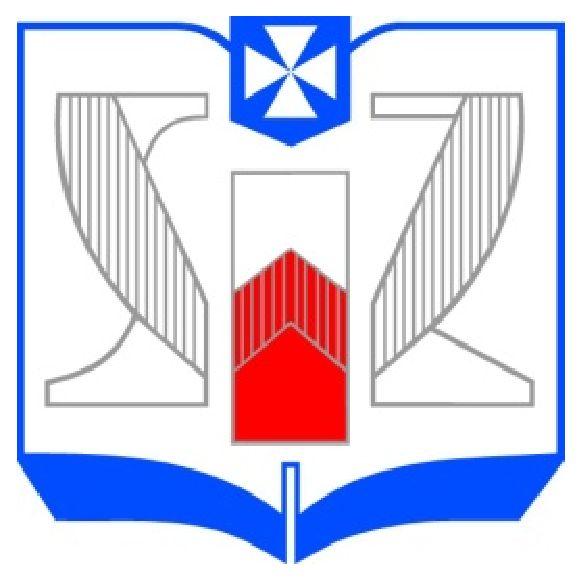
\includegraphics[width=13.0cm, height=3.0cm]{logoWSIiZ}}

\vspace{10mm}
\begin{center}
{\Large{}\textbf{\wydzial}}
\end{center}
\vspace{10mm}
\noindent
\hspace{30mm}{\Large{}\textbf{\kierunek}}\\

\noindent
\hspace{30mm}{\Large{}\textbf{\specjalnosc}}
\vspace{30mm}
\begin{center}
	{\large{}\autor}\\
	{\large{}\album}\\
	\vspace{15pt}
	{\huge{}\textbf{\textit{\temat}}}\\
	\vspace{20pt}
	{\normalsize{}Prowadzący: \promotor}\\
	\vspace{100pt}
	{\LARGE{}\textbf{\typpracy}}\\
	\vspace{190pt}
	{\large{}\textbf{\miasto {} \rok}}
\end{center}

% pusta zawartość stopki - brak numeru strony
\thispagestyle{empty}

% *************** Strona z oświadczeniem o treści pracy ***************
\newpage
\text{}

\thispagestyle{empty}
\newpage


% *************** Spis treści ***************
\tableofcontents
% pusta zawartość stopki - brak numeru strony
\thispagestyle{empty}
\newpage

% *************** Koniec pliku front.tex ***************



% *************** Część główna pracy ***************
\chapter*{Wstęp}


W dobie cyfrowej rewolucji muzycznej, gdzie dostęp do ulubionych utworów stał się niemal nieograniczony, nasze codzienne życie coraz częściej opiera się na dźwiękach płynących z różnorodnych urządzeń. W tym dynamicznie rozwijającym się świecie, Projekt "Music Player" wyróżnia się swoim ambitnym celem – stworzeniem nowoczesnej, wieloplatformowej aplikacji do odtwarzania muzyki, która harmonijnie połączy w sobie funkcjonalność, bezpieczeństwo i estetykę.
% Na co dzień wielu współpracowników w biurach spotyka się z pewnymi niedociągnięciami pojawiającymi się na tle drobnych obowiązków domowych, z którymi nie chcieliby spotykać się jeszcze dodatkowo w pracy, a które wynikają z zaniedbań na tym tle innych pracowników. Do takich małych niedociągnięć i zaniedbań obowiązków należy dla przykładu pozostawianie na dłuższy czas naczyń w zlewozmywaku, nie wynoszenie na czas śmieci, które zalegają w koszu przez dłuższy czas. Albo też nieumyty po używaniu ekspres do kawy, niewymienione po wykorzystaniu pojemniki z tuszem w drukarce. Problemem istotnym, a niebędącym bezpośrednio związanym z przedmiotem działalności firmy, jest dbanie o takie szczegóły, a które mogą wpływać na samopoczucie pracowników i atmosferę w firmie. Dlatego, wbrew pozorom, ważne jest odpowiednie zmotywowanie pracowników aby o takie, mimo że drobne obowiązki, dbali na równi z własnym domem, dzięki czemu każdemu współpracownikowi będzie się lepiej pracowało. I tutaj pojawia rozwiązanie naszego zespołu – system, który jednocześnie w jakiś sposób rozwiązuje powyższe zagadnienie, a z drugiej strony jest także formą urozmaicenia i rozrywki w pracy.

% \textcolor{green}{Przykłady wstępów do prac projektowych/naukowych/dyplomowych można znaleść w artykułach/pracach naukowych/dyplomowych dostępnych w sieci (artykuły/prace naukowe) lub w repozytorium uczelni (biblioteka WSIZ Kielanrowa).}
\addcontentsline{toc}{chapter}{Wstęp}
\newpage
% ********** Rozdział 1 **********
\chapter{Opis założeń projektu}
\section{Cele projetu}

Projekt "Music Player" ma na celu stworzenie nowoczesnej aplikacji do odtwarzania muzyki, która będzie funkcjonować zarówno na systemach Windows, jak i Linux. Kluczowym zadaniem jest zapewnienie spójnego i intuicyjnego interfejsu użytkownika, zrealizowanego przy użyciu frameworka Avalonia, co pozwoli na zachowanie jednolitej estetyki i funkcjonalności na różnych platformach. Aplikacja zostanie napisana w języku C\# z wykorzystaniem środowiska .NET 6, co zagwarantuje jej nowoczesność oraz wysoką wydajność.

Istotną częścią projektu jest wdrożenie systemu logowania, który nie tylko zwiększy bezpieczeństwo i prywatność użytkowników, ale także umożliwi personalizację aplikacji. Dzięki temu użytkownicy będą mogli lepiej zarządzać swoimi playlistami i preferencjami muzycznymi.

Projekt zakłada również opracowanie skutecznego systemu zarządzania danymi baz danych SQL. To umożliwi efektywne przechowywanie informacji o utworach muzycznych, artystach i playlistach. Aplikacja będzie zawierać pełny zestaw funkcji CRUD, co pozwoli użytkownikom na tworzenie, czytanie, aktualizowanie i usuwanie danych w prosty i intuicyjny sposób. Zarządzanie tymi funkcjami zostanie zrealizowane przez starannie zaprojektowaną hierarchię klas, co zapewni logiczną organizację i łatwość w rozwijaniu aplikacji. Znaczącą częścią projektu będzie również rozbudowana obsługa wyjątków oraz mechanizmy walidacji danych, które zagwarantują stabilność aplikacji oraz poprawność przetwarzanych informacji.

Podsumowując, głównym celem projektu "Music Player" jest stworzenie użytecznej, bezpiecznej i przyjaznej dla użytkownika aplikacji do odtwarzania muzyki, która będzie dostosowana do potrzeb użytkowników na różnych platformach, jednocześnie oferując zaawansowane opcje zarządzania zawartością muzyczną.

\section{Założenia projektu}

\begin{itemize}
\item Wieloplatformowość: Aplikacja będzie kompatybilna zarówno z systemami Windows, jak i Linux.
\item Technologie: Wykorzystanie języka programowania C\# oraz frameworka .NET 6.
\item Interfejs Użytkownika: Stworzenie interfejsu graficznego z użyciem Avalonia, zapewniającego spójność i intuicyjność obsługi na różnych platformach.
\item Baza Danych: Początkowe użycie plików tekstowych jako bazy danych, z możliwością rozbudowy do systemu bazodanowego takiego jak SQL.
\item Zarządzanie Danymi: Implementacja funkcjonalności CRUD (Create, Read, Update, Delete) 
\item Walidacja Danych: Weryfikacja poprawności danych wejściowych.
\item Obsługa Wyjątków: Zapewnienie mechanizmów do obsługi błędów i wyjątków w aplikacji.
\item Rozszerzalność: Możliwość rozbudowy aplikacji o dodatkowe funkcje, takie jak importowanie i eksportowanie danych z plików csv.
\item Repozytorium Kodu: Utrzymanie i zarządzanie kodem źródłowym w publicznym repozytorium, np. na GitHub.
\end{itemize}


\section{Wymagania funkcjonale i niefunkcjonalne}

\noindent \textbf{Wymagania funkcjonalne:}

\begin{itemize}
\item Wieloplatformowość: Aplikacja będzie kompatybilna zarówno z systemami Windows, jak i Linux.
\item Technologie: Wykorzystanie języka programowania C\# oraz frameworka .NET 6.
\item Interfejs Użytkownika: Stworzenie interfejsu graficznego z użyciem Avalonia, zapewniającego spójność i intuicyjność obsługi na różnych platformach.
\item Baza Danych: Aplikacja zapewni zaawansowane możliwości zarządzania danymi w bazie SQL, umożliwiając efektywną organizację, aktualizację oraz optymalizację przechowywanych informacji.
\item Zarządzanie Danymi: Implementacja funkcjonalności CRUD (Create, Read, Update, Delete) 
\item Walidacja Danych: Weryfikacja poprawności danych wejściowych.
\item Obsługa Wyjątków: Zapewnienie mechanizmów do obsługi błędów i wyjątków w aplikacji.
\item Rozszerzalność: Możliwość rozbudowy aplikacji o dodatkowe funkcje, takie jak importowanie i eksportowanie danych z plików csv.
\item Repozytorium Kodu: Utrzymanie i zarządzanie kodem źródłowym w publicznym repozytorium, np. na GitHub.
\item Migracja danych: Aplikacja umożliwi efektywną migrację danych z istniejących baz SQL do nowego systemu, wspierając bezproblemowy transfer danych.
\end{itemize}

\noindent \textbf{Wymagania niefunkcjonalne:}

\begin{itemize}
\item Wydajność: Aplikacja powinna szybko reagować na działania użytkownika i efektywnie zarządzać zasobami systemu.
\item Kompatybilność: Działanie na różnych systemach operacyjnych (Windows, Linux) bez konieczności modyfikacji.
\item Bezpieczeństwo: Zabezpieczenie danych użytkownika i systemu przed nieautoryzowanym dostępem.
\item Skalowalność: Możliwość rozbudowy aplikacji o nowe funkcje bez wpływu na istniejącą funkcjonalność.
\item Łatwość Użytkowania: Intuicyjny i prosty w obsłudze interfejs użytkownika.
\item Stabilność: Aplikacja powinna być stabilna i wolna od krytycznych błędów.
\item Dostępność: Łatwość dostępu do aplikacji i jej funkcji dla różnych grup użytkowników.
\item Dokumentacja: Zapewnienie kompletnej i zrozumiałej dokumentacji użytkownika i technicznej.
\end{itemize}

% \noindent \textbf{Wymagania funkcjonalne}
% \begin{itemize}
%     \item opisują funkcje (czynności, operacje, usługi) wykonywane przez system
%     \item Często stosowany sposób opisu wymagań – język naturalny
%     \item Liczba wymagań funkcjonalnych może być bardzo duża; konieczne jest pewnego rodzaju uporządkowanie tych wymagań, które ułatwi pracę nad nimi (złożoność !) 
%     \item Opisują, jak funkcja powinna działać.
%     \item Skupiają się na wyniku działania użytkownika.
%     \item Definiuje wymagania użytkownika.
%     \item Posiada funkcje uwzględnione w przypadkach użycia.
%     \item Weryfikuje funkcjonalność system
% \end{itemize}

% \noindent \textbf{Wymagania niefunkcjonalne }
% \begin{itemize}
%     \item opisują ograniczenia, przy zachowaniu których system powinien realizować swe funkcje.     
%     \item Opisują, jakie właściwości sprawią, że funkcja będzie działać.
%     \item Skupiają się na uproszczeniu procesu i wykonania wyniku.
%     \item Definiują oczekiwania i doświadczenia użytkownika działania użytkownika.
%     \item Posiadają ograniczenia, które pomogą zredukować czas i koszty rozwoju.
%     \item Weryfikują wydajność systemu.
% \end{itemize}
 
% \noindent \textbf{Wymagania funkcjonalne przykłady:}

% Lista przykładów wymagań funkcjonalnych obejmuje każde zachowanie systemu IT, zmieniające się pod wpływem zastosowanej funkcji. Jeżeli wymagania funkcjonalne nie zostaną potwierdzone, system nie będzie działał.
% \begin{itemize}
%     \item Reguły biznesowe.
%     \item Poziomy autoryzacji.
%     \item  Śledzenie audytów.
%     \item Interfejsy zewnętrzne.
%     \item Funkcje administracyjne.
%     \item Generowanie danych historycznych.
%     \item Uwierzytelnianie użytkownika na żądanie.
%     \item Logi serwera wszystkich istniejących danych.
%     \item Generowanie raportów w określonym czasie.
%     \item Definiowanie poziomów autoryzacji systemu.
% \end{itemize}

% \noindent \textbf{Wymagania niefunkcjonalne przykłady:}

% \noindent Na liście wymagań niefunkcjonalnych znajdują się,
% \begin{itemize}
%     \item Pojemność.
%     \item Wydajność.
%     \item Środowisko.
%     \item Użyteczność.
%     \item Skalowalność.
%     \item  Niezawodność.
%     \item Odzyskiwalność.
%     \item Bezpieczeństwo.
%     \item Utrzymywalność.
%     \item Interoperacyjność.
%     \item Integralność danych.
%     \item  2-poziomowe uwierzytelnianie.
% \end{itemize}

% \noindent Rozwinięcie wymagań niefunkcjonalnych:
% \begin{itemize}
%     \item Aplikacja IT powinna mieć kolor tła wszystkich ekranów \#fffaaa.
%     \item Aplikacja IT powinna przestrzegać wymagań regulatora.
%     \item Aplikacja IT powinien rejestrować każdą nieudaną próbę logowania;
%     \item Użytkownicy powinni zmienić hasło po pierwszym udanym logowaniu.
%     \item  Dashboard powinien pojawić się w ciągu 3 sekund po zalogowaniu użytkownika.
%     \item Aplikacja IT powinien być w stanie obsłużyć XYZ liczbę użytkowników, zapewniając płynne działanie.
% \end{itemize}

% Jak zdefiniować wymagania funkcjonalne?

% Jeśli twoje podejście do rozwoju oprogramowania jest zwinne (Agile), prawdopodobnie zdefiniujesz wymagania w dokumencie. Dokument wymagań funkcjonalnych będzie zawierał historie użytkowników, przypadki użycia, a także następujące sekcje.
% \begin{itemize}
%     \item Cel: Ta sekcja będzie zawierała całe tło, definicje i przegląd systemu;
%     \item Zakres aplikacji, oczekiwania i zasady biznesowe;
%     \item Wymagania dotyczące bazy danych, atrybuty systemu i wymagania funkcjonalne;
%     \item Przypadki użycia, czyli opisywać, w jaki sposób użytkownik będzie wchodził w interakcję z systemem. Zdefiniuj rolę każdego aktora biorącego udział w interakcji;
%     \item Napisz jasno cel wdrożenia systemu IT.
%     \item Wspomnij o użytkownikach aplikacji, którzy szczegółowo opiszą, jak krok po kroku będą się angażowali w tworzenie aplikacji.
%     \item Opracuj klikalny prototyp aplikacji. To pomoże Ci reprezentować produkt w lepszy i przekonujący sposób dla interesariuszy. Możesz wybrać prototypy do wyrzucenia lub prototypy interaktywne dla swojego projektu.
% \end{itemize}

% \noindent Jak zdefiniować wymaganie niefunkcjonalne?

% Teraz nadchodzi część, w której definiujesz oczekiwania jakościowe aplikacji dedykowanej. Te atrybuty opisują sposoby, w jakie oczekujesz, że aplikacja będzie się zachowywała.
% \begin{itemize}
%     \item Zdefiniuj oczekiwania dotyczące użyteczności produktu.
%     \item Opisz, do jakich praw i regulacji aplikacja powinna spełniać.
%     \item Zdefiniuj dostępność aplikacji, czyli czy będzie ona funkcjonować 24/7/365?
%     \item Określ wydajność systemu IT dla różnych funkcjonalności. To znaczy, w jakim czasie użytkownik powinien zobaczyć listę, jak długo użytkownik będzie połączony z aplikacją w przypadku braku połączenia z internetem, itp.
%     \item Zdefiniuj wymagania dotyczące bezpieczeństwa systemu IT.
%     \item Użyj narzędzi do automatycznego testowania, aby upewnić się co do wydajności aplikacji dedykowanej.
% \end{itemize}


% \subsection{Przkłady}

% \noindent Przykłady wymagań funkcjonalnych aplikacji webowej:
% \begin{itemize}
%     \item Rejestracja i logowanie użytkowników.
%     \item Bezpieczne uwierzytelnianie i autoryzacja użytkowników.
%     \item Zarządzanie profilami użytkowników.
%     \item Możliwość wyszukiwania treści w aplikacji.
%     \item Funkcjonalność e-commerce, taka jak koszyk i proces kasowy.
%     \item Treści generowane przez użytkowników, takie jak komentarze i oceny.
%     \item Integracja z usługami stron trzecich, takimi jak media społecznościowe i bramki płatności.
%     \item Dynamiczne aktualizacje treści i powiadomienia.
%     \item Pulpit administracyjny do zarządzania aplikacją.
% \end{itemize}
% \noindent Przykłady wymagań niefunkcjonalnych aplikacji webowej:
% \begin{itemize}
%     \item Użyteczność aplikacji i dostępność, takie jak responsywny design i dostępność klawiatury.
%     \item Wydajność aplikacji i skalowalność, np. szybkie czasy ładowania i zdolność do obsługi dużej liczby użytkowników jednocześnie.
%     \item Bezpieczeństwo aplikacji i prywatność, takie jak szyfrowanie wrażliwych danych i ochrona przed atakami.
%     \item Niezawodność aplikacji i dostępność, np. kopie zapasowe i plany odzyskiwania danych po awarii.
%     \item Zgodność aplikacji z wymogami prawnymi i regulacyjnymi, takimi jak GDPR i przepisy dotyczące dostępności.
%     \item Interoperacyjność aplikacji, taka jak zgodność z różnymi przeglądarkami i systemami operacyjnymi.
%     \item Utrzymanie i wsparcie aplikacji, takie jak łatwość aktualizacji i dokumentacja dla programistów.
%     \item Efektywność kosztowa aplikacji, taka jak minimalizacja kosztów serwera i hostingu.
% \end{itemize}
% System zarządzania treścią (CMS) umożliwiający edycję i usuwanie treści.

% \noindent Przykłady wymagań funkcjonalnych aplikacji webowej:
% \begin{itemize}
%     \item Integracja aplikacji z zewnętrznymi API w celu wymiany danych lub rozszerzenia funkcjonalności.
%     \item Funkcje optymalizacji aplikacji pod kątem wyszukiwarek (SEO) w celu poprawy widoczności w wyszukiwarkach internetowych.
%     \item Obsługa wielu języków w aplikacji w celu dostosowania do użytkowników posługujących się różnymi językami.
%     \item Narzędzia współpracy, takie jak czat w czasie rzeczywistym i udostępnianie plików dla zespołów.
%     \item Narzędzia analizy danych do śledzenia zachowań użytkowników i wydajności aplikacji.
% \end{itemize}
% Projektowanie doświadczeń użytkownika (UX), takich jak łatwy w użyciu interfejs i przejrzysta nawigacja.

% \noindent Przykłady wymagań niefunkcjonalnych aplikacji webowej:
% \begin{itemize}
%     \item Optymalizacja mobilna aplikacji, np. responsywny design i podejście mobile-first.
%     \item Integracja systemu, np. kompatybilność z dotychczasowymi systemami i narzędziami stron trzecich.
%     \item Bezpieczeństwo aplikacji i prywatność danych, takie jak szyfrowanie danych, kopie zapasowe i kontrola dostępu.
%     \item Zgodność aplikacji z normami branżowymi, takimi jak PCI-DSS dla aplikacji e-commerce.
%     \item Wsparcie dla użytkowników aplikacji, takie jak help desk, podręczniki użytkownika i samouczki.
%     \item Monitorowanie aplikacji i raportowanie, takie jak śledzenie błędów i metryki wydajności.
% \end{itemize}

% To tylko kilka przykładów funkcjonalnych i niefunkcjonalnych wymagań aplikacji internetowych. Konkretne wymagania będą zależały od celu i charakteru aplikacji internetowej, a także potrzeb użytkowników i zainteresowanych stron.


% ********** Koniec rozdziału **********

\newpage
% ********** Rozdział 2 **********
\chapter{Opis struktury projektu}

{Projekt ten został zrealizowany z wykorzystaniem nowoczesnych technologii programistycznych. Głównym językiem programowania jest C\#, znany ze swojej wszechstronności i wydajności, co czyni go idealnym wyborem dla aplikacji multimedialnych. Aplikacja korzysta z frameworka Entity Framework do zarządzania bazą danych, co pozwala na efektywne i bezproblemowe przechowywanie oraz dostęp do danych użytkownika. Interfejs użytkownika został zbudowany z wykorzystaniem Avalonia, nowoczesnego frameworka GUI, który zapewnia płynne i atrakcyjne wizualnie doświadczenie użytkownika.}

\section{Kluczowe Technologie i Narzędzia w Projekcie}

\begin{itemize}
    \item \textbf{ .NET 6:}  Jako kompleksowe środowisko uruchomieniowe i framework programistyczny, .NET 6 oferuje wydajność, bezpieczeństwo i wsparcie dla wielu platform, co jest niezbędne dla nowoczesnych aplikacji. Umożliwia ono tworzenie wydajnej i skalowalnej aplikacji, zapewniając jednocześnie wsparcie dla najnowszych standardów i praktyk programistycznych.
    \item \textbf{ Avalonia :} Jest frameworkiem do tworzenia interfejsów użytkownika, który umożliwia tworzenie aplikacji działających na wielu platformach. W projekcie "Music Player", Avalonia jest wykorzystywana do stworzenia atrakcyjnego i responsywnego interfejsu użytkownika, który jest spójny na różnych systemach operacyjnych. Dzięki swojej elastyczności i wsparciu dla XAML, Avalonia idealnie nadaje się do budowy nowoczesnych aplikacji multimedialnych, takich jak "Music Player", oferując zaawansowane funkcje GUI, takie jak animacje, style i szablony.
    
    \item \textbf{ Repozytorium kodu Github:}  Jest to platforma do hostingu kodu źródłowego, która wykorzystuje system kontroli wersji Git. Umożliwia przechowywanie, zarządzanie i śledzenie zmian w kodzie projektów. 
    \item \textbf{ GitHub Actions:} Jest to narzędzie CI/CD (Continuous Integration/Continuous Deployment) zintegrowane z GitHubem, które umożliwia automatyzację różnych etapów rozwoju oprogramowania, takich jak testowanie, budowanie i wdrażanie aplikacji. W projekcie "Music Player", GitHub Actions jest używany do automatycznego budowania projektu, co jest widoczne w pliku dotnet-build.yml. Ten plik definiuje zadania, które są wykonywane automatycznie przy każdym pushu lub pull requeście, zapewniając ciągłą integrację i sprawdzanie jakości kodu.
    \item \textbf{ Baza Danych MySQL:} Jest to popularny system zarządzania relacyjnymi bazami danych (RDBMS). Charakteryzuje się otwartym źródłem i jest szeroko stosowany w aplikacjach internetowych. W projekcie "Music Player", MySQL używany jest do przechowywania danych użytkowników, playlist, utworów i plików muzycznych. Jest to wybór odpowiedni dla aplikacji wymagających niezawodnego, skalowalnego i łatwego w zarządzaniu systemu bazodanowego.
    \item \textbf{ Docker i Docker Compose:}  Używane są do zarządzania lokalnym środowiskiem serwera SQL, co ułatwia testowanie i rozwój aplikacji. Docker pozwala na szybkie uruchomienie izolowanego środowiska MySQL, a Docker Compose upraszcza konfigurację i zarządzanie wieloma kontenerami. Ta kombinacja narzędzi zapewnia wydajne i elastyczne środowisko deweloperskie, które jest kluczowe dla płynnego rozwoju projektu.
    \item \textbf{ JetBrains DataGrid:} Jest to kontrolka interfejsu użytkownika umożliwiająca efektywne wyświetlanie i manipulowanie danymi w formie tabeli. W "Music Player" DataGrid jest wykorzystywany do prezentacji i zarządzania informacjami, takimi jak listy utworów czy dane użytkowników od strony administratora.
    \item \textbf{ JetBrains Rider:}  Jest zaawansowanym zintegrowanym środowiskiem programistycznym (IDE) dla platformy .NET, które oferuje bogate funkcje, takie jak refaktoryzacja, inteligentne podpowiedzi kodu i efektywne debugowanie.
    \item \textbf{ Visual Studio: } Z kolei, zostało użyte do wygenerowania diagramu klas, co pomaga wizualizować strukturę i zależności między różnymi komponentami aplikacji. Użycie Visual Studio do tworzenia diagramów klas jest przydatne w celu lepszego zrozumienia architektury projektu.
    
\end{itemize}


\section{Narzędzia i Rozszerzenia NuGet}

Projekt "Music Player" wykorzystuje szereg rozszerzeń NuGet, które znacząco przyczyniają się do jego funkcjonalności i wydajności. Poniżej przedstawiam szczegółowy opis każdego z tych pakietów:

\begin{enumerate}
    \item \textbf{ Avalonia:} (W tym: Avalonia.Desktop, Avalonia.Themes.Fluent i  Avalonia.Fonts.Inter) Są to główne pakiety frameworka GUI używany w projekcie. Avalonia umożliwia tworzenie atrakcyjnych, platformowo niezależnych interfejsów użytkownika. Jest to kluczowy element, który pozwala aplikacji działać na różnych systemach operacyjnych.
    \item \textbf{ CsvHelper:} Biblioteka ta ułatwia operacje na plikach CSV, takie jak ich czytanie i zapisywanie. Jest to przydatne w kontekście eksportowania lub importowania danych, np. list utworów.
    \item \textbf{Microsoft.EntityFrameworkCore:} Jest to framework ORM (Object-Relational Mapping) od Microsoftu, który umożliwia efektywne zarządzanie bazą danych w sposób obiektowy. Jest kluczowy dla operacji CRUD (Create, Read, Update, Delete) w projekcie.
    
    \item \textbf{Microsoft.EntityFrameworkCore.Tools:} Zestaw narzędzi wspierających Entity Framework Core, w tym migracje bazy danych, co jest istotne dla utrzymania i aktualizacji struktury bazy danych.
    
    \item \textbf{NAudio:} Jest to biblioteka do obsługi dźwięku, która pozwala na odtwarzanie, nagrywanie, edycję i konwersję plików audio. Jest kluczowa dla funkcjonalności odtwarzacza muzyki w projekcie.
    
    \item \textbf{Pomelo.EntityFrameworkCore.MySql:} Ten pakiet umożliwia wykorzystanie MySQL jako bazy danych w połączeniu z Entity Framework Core, co zapewnia wsparcie dla popularnego systemu zarządzania bazą danych MySQL.
\end{enumerate}

Każdy z tych pakietów odgrywa istotną rolę w funkcjonowaniu aplikacji "Music Player", zapewniając niezbędne narzędzia i funkcje, które przyczyniają się do jej wydajności, stabilności i atrakcyjności użytkowej.

\newpage

\section{Minimalne wymagania systemowe}

\paragraph{Wymagania minimalne dla systemu Windows:}

\begin{enumerate}
    \item \textbf{ System Operacyjny:} Windows 10.
    \item \textbf{ Procesor:} Intel Core i3 (8. generacji) lub nowszy / AMD Ryzen 3 (2. generacji) lub nowszy, z co najmniej 4 rdzeniami.
    \item \textbf{ Pamięć RAM:} Minimum 6 GB.
    \item \textbf{ Miejsce na Dysku:} Minimum 500 MB wolnego miejsca na dysku twardym.
    \item \textbf{ .NET Runtime:} .NET Core 6.0 lub nowszy.
    \item \textbf{ Dźwięk:} Karta dźwiękowa kompatybilna z systemem operacyjnym.
    \item \textbf{ Karta Graficzna:} Wsparcie dla DirectX 9 lub nowszego z WDDM 1.0 driver.
\end{enumerate}

\paragraph{Wymagania minimalne dla systemu Linux:}

\begin{enumerate}
    \item \textbf{ System Operacyjny:} Ubuntu 16.04 lub nowsza, Fedora 29 lub nowsza, Debian 9 lub nowsza, lub inne kompatybilne dystrybucje.
    \item \textbf{ Procesor:} Intel Core i3 (8. generacji) lub nowszy / AMD Ryzen 3 (2. generacji) lub nowszy, z co najmniej 4 rdzeniami.
    \item \textbf{ Pamięć RAM:}  Minimum 4 GB.
    \item \textbf{ Miejsce na Dysku:} Minimum 500 MB wolnego miejsca.
    \item \textbf{ .NET Runtime:} .NET Core 6.0 lub nowszy.
    \item \textbf{ Dźwięk:} Karta dźwiękowa kompatybilna z systemem operacyjnym.
    \item \textbf{ Biblioteki:} libgtk-3-0, libwebkit2gtk-4.0-37, libasound2 (dla Ubuntu/Debian), libX11, libXtst, libXScrnSaver, libsecret-1-0, libc6, libgcc1, libgdiplus (dla Fedora).
    
\end{enumerate}




\section{Zaprojektowana Struktura i Opis Techniczny}

Projekt "Music Player" reprezentuje zaawansowane podejście do programowania aplikacji, łącząc w sobie najlepsze praktyki i wzorce projektowe. Składający się z 48 klas, w tym 4 interfejsów i 2 enumów, projekt ten jest doskonałym przykładem efektywnego wykorzystania architektury opartej na luźno powiązanych klasach, co jest możliwe dzięki zastosowaniu Dependency Injection (DI) oraz wzorca Singleton.


\newpage
\textbf{Diagram klas projektu}

\begin{figure}[!ht]
	\begin{center}
	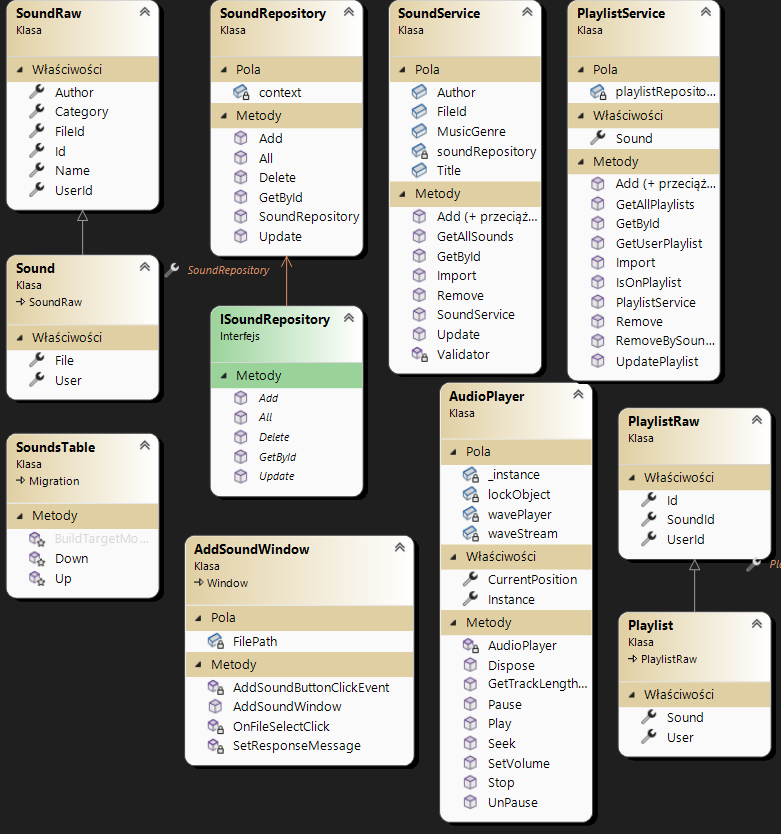
\includegraphics[width=500pt]{figures/diagram_cz1.png}
        \caption{{\footnotesize Diagram klas cześć 1}}
	\end{center}
\end{figure}


{Na przedstawionym diagramie widzimy tylko część klas projektu (jedną z czterech części całego diagramu). Rozmieszczenie tych klas nie jest bezpośrednio związane, gdyż obejmuje zarówno klasy repozytorium bazy danych, serwisy, pomocnicze klasy do migracji takie jak \texttt{SoundsTable}, jak i klasy tworzące interfejs użytkownika GUI, na przykład \texttt{AddSoundWindow}. Interesujące może być zastosowanie dziedziczenia klasy \texttt{SoundRaw} w klasie \texttt{Sound}. Rozwiązanie to jest stosowane tylko w wybranych przypadkach. Klasa \texttt{Sound} reprezentuje tabelę \texttt{Sounds}, o której będzie mowa później, ale definiuje również obiekty takie jak \texttt{File} oraz \texttt{User}, które są używane w relacjach między tabelami w bazie danych. Klasa \texttt{SoundRaw} definiuje wyłącznie kolumny w bazie (nie uwzględnia relacji), co jest potrzebne w kontekście importu i eksportu danych do formatu CSV.

Kolejnym interesującym aspektem jest zastosowanie wzorca Dependency Injection do wstrzykiwania klasy repozytorium \texttt{SoundRepository} w konstruktorze serwisu \texttt{SoundService}. Interfejs \texttt{ISoundRepository} definiuje metody, które nasze \texttt{SoundRepository} implementuje, a następnie instancja tego repozytorium jest wstrzykiwana do serwisu.



Klasa \texttt{SoundService} oferuje wszechstronne zarządzanie danymi, w tym operacje CRUD, walidację danych, import i eksport, a także obsługę błędów. Podobnie klasa \texttt{PlaylistService} umożliwia wykonanie tych samych operacji, jednak nie zajmuje się walidacją danych, gdyż nie operuje na danych wprowadzonych przez użytkownika, co sprawia, że jej obsługa jest nieco prostsza. Kolejnym kluczowym elementem przedstawionego diagramu jest klasa \texttt{AudioPlayer} – to ona przetwarza, odtwarza i zarządza dźwiękiem w aplikacji. Dysponuje metodami takimi jak \texttt{GetTrackLengthInSeconds()}, która zwraca długość aktualnie odtwarzanego utworu w sekundach, \texttt{SetVolume()} do regulacji głośności, a także \texttt{Play()}, \texttt{Stop()} i \texttt{Pause()} do kontrolowania odtwarzania utworu.
}

\begin{figure}[!ht]
	\begin{center}
	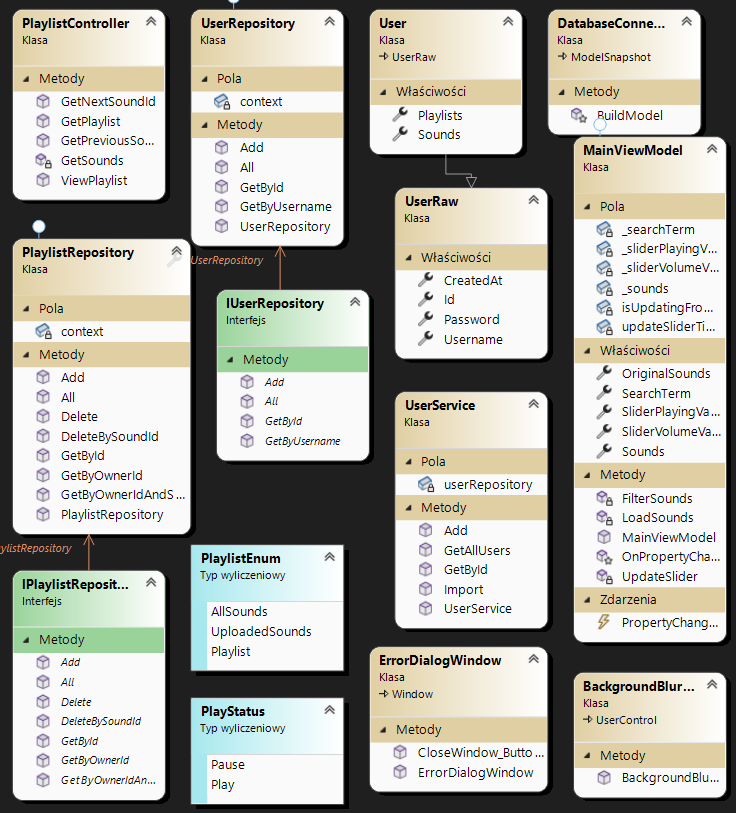
\includegraphics[width=500pt]{figures/diagram_czesc2.png}
        \caption{{\footnotesize Diagram klas cześć 2}}
	\end{center}
\end{figure}

\newpage

{Na kolejnym, drugim już diagramie, główną uwagę przykuwa klasa \texttt{MainViewModel}, która odpowiada za zarządzanie danymi między interfejsem użytkownika (UI) a logiką aplikacji. Odpowiada ona za odtwarzanie, wyszukiwanie, przewijanie, regulację głośności oraz kontrolowanie utworów. Opis reszty klas przedstawiono w punktach:}

\begin{enumerate}
    \item \textbf{ PlaylistController:} Klasa kontrolera zarządzająca playlistami. Posiada metody takie jak \newline \texttt{GetNextSoundId}, \texttt{GetPlaylist}, \texttt{GetPreviousSoundId}, \texttt{GetSounds}, \texttt{ViewPlaylist}, które służą do nawigacji i zarządzania listami odtwarzania w interfejsie użytkownika.
    \item \textbf{ UserRepository:} Repozytorium obsługujące operacje na danych użytkowników. Zawiera pola i metody niezbędne do realizacji operacji CRUD na użytkownikach, takie jak \texttt{Add}, \texttt{All}, \texttt{Delete}, \texttt{GetById}, \texttt{GetByUsername}.
    \item \textbf{ IUserRepository:}  Interfejs definiujący metody dostępu do danych użytkowników, których implementacja jest wymagana w \texttt{UserRepository}.
    \item \textbf{ User i UserRaw:} \texttt{User} definiuje tablice \texttt{Users} w bazie danych z relacją do tablic \texttt{Playlists} i \texttt{Sounds}. \texttt{UserRaw} reprezentuje surowe dane użytkownika, takie jak \texttt{Id}, \texttt{Password}, \texttt{Username}.
    \item \textbf{ UserService:} Serwis zapewniający logikę biznesową związaną z użytkownikami. Posiada pola i metody, takie jak \texttt{Add}, \texttt{GetAllUsers}, \texttt{GetById}, \texttt{Import}, które pozwalają na zarządzanie danymi użytkowników.
    \item \textbf{ DatabaseConnectionContextModelSnapshot:} Klasa \texttt{ModelSnapshot}, która zarządza wersjonowaniem modelu bazy danych..
    \item \textbf{ PlaylistRepository i IPlaylistRepository:}  Analogicznie do \texttt{UserRepository}, te klasy zarządzają operacjami na playlistach, z metodami do wykonania operacji CRUD.
    \item \textbf{ PlaylistEnum i PlayStatus:}  Typy wyliczeniowe, które definiują zbiór wartości, jakie mogą przyjąć playlisty (\texttt{AllSounds, UploadedSounds, Playlist}) oraz statusy odtwarzania (\texttt{Pause, Play}).
    \item \textbf{ ErrorDialogWindow:}  Klasa okna dialogowego służąca do wyświetlania komunikatów o błędach, posiada metodę taką jak \texttt{CloseWindow\_ButtonClick}.
    \item \textbf{ BackgroundBlur:}  Klasa \texttt{UserControl}, która służy do dodawania efektu rozmycia tła w interfejsie użytkownika.
\end{enumerate}

\begin{figure}[!ht]
	\begin{center}
	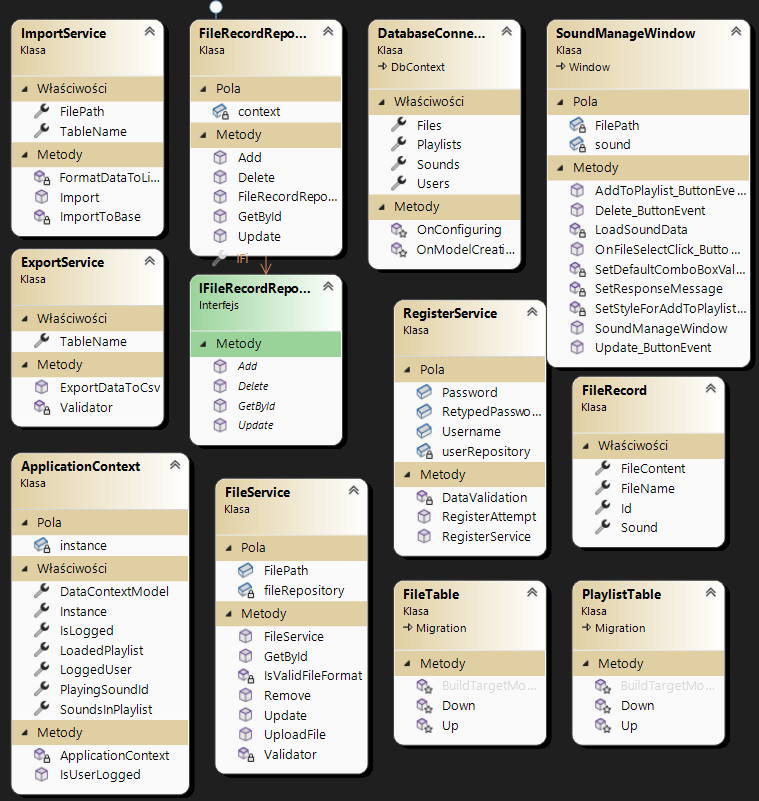
\includegraphics[width=500pt]{figures/diagram_czesc3.png}
        \caption{{\footnotesize Diagram klas cześć 3}}
	\end{center}
\end{figure}

\newpage
{Przedostatnia część diagramu, czyli trzecia, prezentuje nam klasę \texttt{ApplicationContext}. Klasa ta służy jako centralny punkt zarządzania stanem aplikacji i zawiera informacje o zalogowanym użytkowniku, załadowanej playliście i odtwarzanym dźwięku. Wykorzystuje ona wzorzec projektowy \texttt{Singleton}, który zapewnia stworzenie tylko jednej instancji klasy, co pozwala efektywnie przechowywać stan aplikacji. Opis reszty klas: }

\begin{enumerate}
    \item \textbf{ ImportService:} Klasa służąca do importowania danych. Posiada właściwości takie jak \texttt{FilePath} i \texttt{TableName}, a także metody \texttt{FormatDataToList}, \texttt{Import}, \texttt{ImportToBase}, które pozwalają na przetwarzanie i załadowanie danych do bazy danych.
    \item \textbf{ FileRecordRepository:} Repozytorium obsługujące operacje na rekordach plików. Zawiera standardowe metody CRUD: \texttt{Add}, \texttt{Delete}, \texttt{GetById}, \texttt{Update}.
    \item \textbf{ IFileRecordRepository:} Interfejs definiujący kontrakt dla \texttt{FileRecordRepository}, zapewniając oddzielenie implementacji od abstrakcji.
    \item \textbf{ ExportService:} Klasa odpowiedzialna za eksport danych. Posiada metody takie jak \newline \texttt{ExportDataToCsv} oraz \texttt{Validator}, które pozwalają na weryfikację i eksport danych do formatu CSV.
    \item \textbf{ DatabaseConnection:} Klasa z rozszerzeniem \texttt{DbContext}, używana przez Entity Framework do konfiguracji połączenia z bazą danych oraz definiowania modelu bazy danych za pomocą metod \texttt{OnConfiguring} i \texttt{OnModelCreating}.
    \item \textbf{ SoundManageWindow:} Klasa reprezentująca okno zarządzania dźwiękiem w interfejsie użytkownika. Zawiera metody do dodawania dźwięków do playlisty, usuwania, ładowania danych dźwiękowych, aktualizacji i innych interakcji z użytkownikiem.
    \item \textbf{ RegisterService:} Serwis obsługujący rejestrację użytkowników. Wykorzystuje \texttt{userRepository} do dostępu do danych użytkowników i zawiera metody \texttt{DataValidation}, \texttt{RegisterAttempt} do walidacji i próby rejestracji.
    \item \textbf{ FileService:} Serwis do zarządzania plikami, z metodami takimi jak \texttt{GetById}, \newline \texttt{IsValidFileFormat}, \texttt{Remove}, \texttt{Update}, \texttt{UploadFile}, \texttt{Validator}.
    \item \textbf{ FileRecord:} Klasa reprezentująca rekord pliku w tabeli \texttt{Files} w bazie danych MySQL z właściwościami takimi jak \texttt{FileContent}, \texttt{FileName}, \texttt{Id}, \texttt{Sound}.
    \item \textbf{ FileTable i PlaylistTable:} Klasy migracji, które są częścią Entity Framework Migrations i zawierają metody Up i Down do aktualizacji schematu bazy danych.
\end{enumerate}

\begin{figure}[!ht]
	\begin{center}
	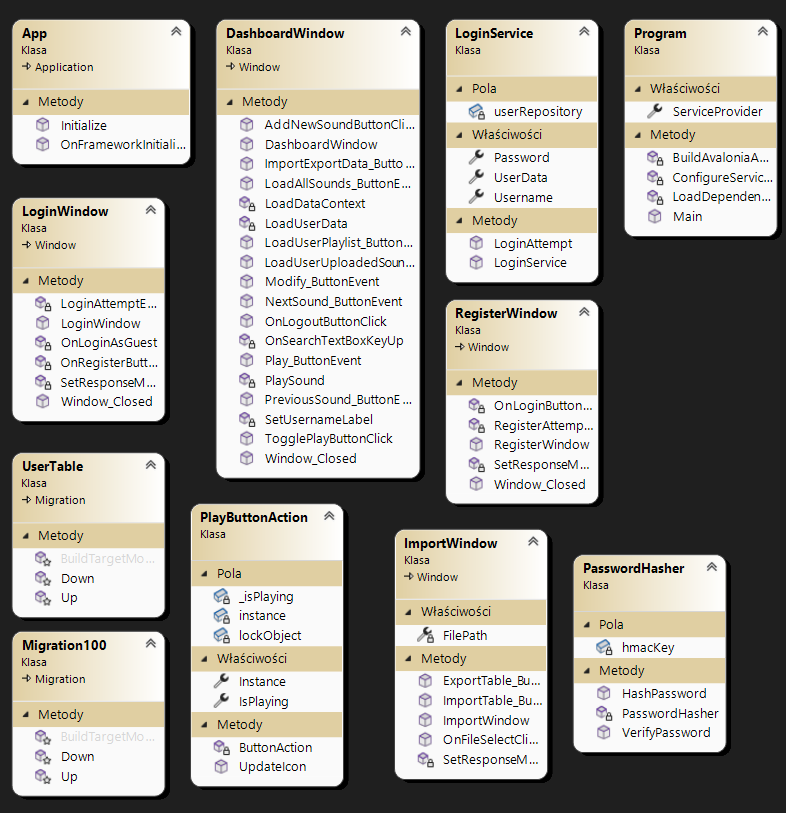
\includegraphics[width=500pt]{figures/diagram_czesc4.png}
        \caption{{\footnotesize Diagram klas cześć 3}}
	\end{center}
\end{figure}

\newpage

{Już ostatnia część diagramu prezentuje klasy takie jak \texttt{Program} (odpowiedzialna za uruchomienie aplikacji), \texttt{App} (inicjalizująca interfejs użytkownika w Avalonii) oraz \texttt{DashboardWindow}. \texttt{DashboardWindow} to klasa reprezentująca główne okno interfejsu użytkownika (Dashboard), przez które użytkownik może zarządzać aplikacją. Zawiera metody do zarządzania dźwiękiem, danymi oraz playlistami, takie jak \texttt{AddNewSoundButtonClickEvent}, \texttt{LoadData}, \texttt{LoadUserData}, \newline \texttt{TogglePlayButtonClick} i inne, co umożliwia interaktywną obsługę różnorodnych funkcji aplikacji. Opis pozostałych klas:}

\begin{enumerate}
    \item \textbf{ LoginService:} Serwis odpowiedzialny za proces logowania. Używa \texttt{userRepository} do dostępu do danych użytkownika i zawiera metody takie jak \texttt{LoginAttempt} do obsługi weryfikacji danych logowania.
    \item \textbf{ RegisterWindow:} Okno do rejestracji nowych użytkowników. Posiada metody takie jak \newline \texttt{OnLoginButtonClick}, \texttt{RegisterAttempt}, co pozwala na obsługę zdarzeń związanych z procesem rejestracji.
    \item \textbf{ UserTable i Migration100:} Klasy reprezentujące migracje bazy danych, używane do aktualizacji schematu bazy danych, z metodami \texttt{Up} i \texttt{Down}.
    \item \textbf{ PlayButtonAction:} Klasa, która zarządza stanem przycisku odtwarzania. Posiada pola określające stan odtwarzania \texttt{\_isPlaying} i metody takie jak \texttt{ButtonAction}, \texttt{UpdateIcon} co wskazuje na możliwość zmiany stanu przycisku odtwarzania.
    Dodatkowo, klasa ta jest tworzona jako pojedyncza instancja zgodnie z wzorcem projektowym Singleton.
    \item \textbf{ ImportWindow:} Okno do importowania danych do aplikacji. Zawiera metody \newline \texttt{ExportTableButtonClickEvent}, \texttt{OnFileSelectClick}, które pozwalają na interakcję z użytkownikiem podczas importowania danych z plików.
    \item \textbf{ PasswordHasher:} Klasa zawierająca metody do hashowania i weryfikacji haseł, takie jak \newline \texttt{HashPassword}, \texttt{VerifyPassword}, co jest istotne dla bezpieczeństwa danych użytkowników.
\end{enumerate}

\section{Zarządzenie danymi w aplikacji}

Schemat bazy danych MySQL wykorzystywanej przez aplikację:

\begin{figure}[!ht]
	\begin{center}
	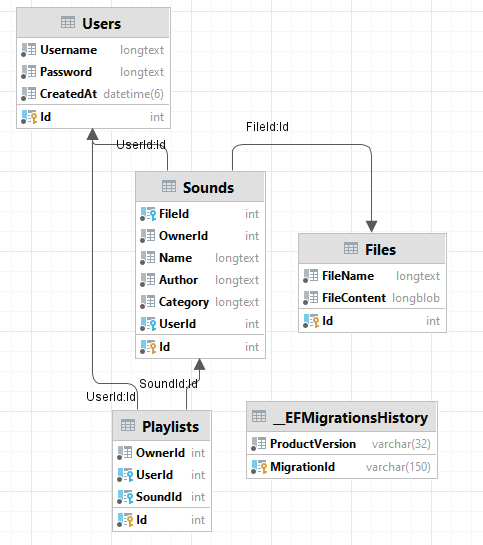
\includegraphics[height=300pt]{figures/schema.png}
        \caption{{\footnotesize Schema bazy danych}}
	\end{center}
\end{figure}

Na załączonym schemacie bazy danych aplikacji widoczne są cztery kluczowe tabele, które współgrają ze sobą, tworząc kompleksowy system zarządzania danymi:



\begin{enumerate}
    \item \textbf{Użytkownicy (Users):} Serce systemu stanowi tabela \texttt{Users}, przechowująca niezbędne informacje o użytkownikach, takie jak nazwa użytkownika (\texttt{Username}), hasło (\texttt{Password}) zahashowane przy pomocy algorytmu HMACSHA512, data utworzenia konta (\texttt{CreatedAt}) oraz unikalny identyfikator (\texttt{Id}). Ta tabela jest fundamentem dla autentykacji oraz zarządzania profilami użytkowników.
    \item \textbf{Dźwięki (Sounds):} Tabela \texttt{Sounds} służy jako repozytorium metadanych dla plików dźwiękowych w aplikacji. Każdy rekord dźwięku zawiera odniesienie do pliku (\texttt{FileId}), identyfikator właściciela (\texttt{OwnerId}), nazwę (\texttt{Name}), autora (\texttt{Author}), kategorię (\texttt{Category}) oraz unikalny identyfikator (\texttt{Id}). Powiązanie z tabelą \texttt{Users} za pomocą \texttt{UserId} umożliwia śledzenie, który użytkownik przesłał dany dźwięk, ułatwiając zarządzanie treścią i prawami własności.
    \item \textbf{Pliki (Files):} W tabeli \texttt{Files} przechowywane są właściwe dane plików dźwiękowych, takie jak zawartość pliku (\texttt{FileContent}) i nazwa pliku (\texttt{FileName}), każdy z unikalnym identyfikatorem (\texttt{Id}). Ta tabela działa jako magazyn danych binarnych, co pozwala na oddzielenie fizycznych plików od ich opisowych metadanych przechowywanych w tabeli Sounds.
    \item \textbf{Playlisty (Playlists):} Użytkownicy mogą tworzyć spersonalizowane playlisty za pośrednictwem tabeli \texttt{Playlists}, która zawiera odniesienia do ich twórców (\texttt{OwnerId}) oraz przypisane dźwięki (\texttt{SoundId}). Każda playlista posiada swój unikalny identyfikator (\texttt{Id}), co umożliwia łatwe odnajdywanie i zarządzanie kolekcjami dźwięków.
    \item \textbf{Historia Migracji EF (EFMigrationsHistory):} Specjalna tabela \texttt{\_EFMigrationsHistory} jest wykorzystywana przez Entity Framework do przechowywania historii migracji, które są niezbędne do aktualizacji i utrzymania integralności schematu bazy danych.

\end{enumerate}

Wszystkie te tabele łączą się w spójny system, który umożliwia dynamiczne zarządzanie danymi użytkowników, ich twórczością oraz preferencjami. Dzięki starannie przemyślanej architekturze i relacjom między tabelami, aplikacja jest w stanie zapewnić efektywne i bezproblemowe doświadczenia dla użytkownika, od logowania i rejestracji, przez przesyłanie i odtwarzanie dźwięków, aż po tworzenie i użytkowanie playlist.

Aplikacja umożliwia również import i eksport danych w formacie CSV, jednakże jest to ograniczone, ponieważ operacje te są problematyczne dla tabeli `Files`. Zawiera ona bardzo duże rekordy, które obejmują całe pliki piosenek. W związku z tym, w obecnej wersji aplikacji, import i eksport tabeli Files nie jest dostępny. Import innych tabel, takich jak `Users`, `Playlists` i `Sounds`, funkcjonuje natomiast bez zarzutu.



% ********** Koniec rozdziału **********

\newpage
% ********** Rozdział 4 **********
\chapter{Harmonogram realizacji projektu}

{W tym rozdziale przedstawiony jest harmonogram realizacji projektu aplikacji muzycznej, "Music Player", opracowanej w języku C\#. Harmonogram ten jest graficznie reprezentowany za pomocą diagramu Gantta: }

\begin{figure}[!ht]
	\begin{center}
	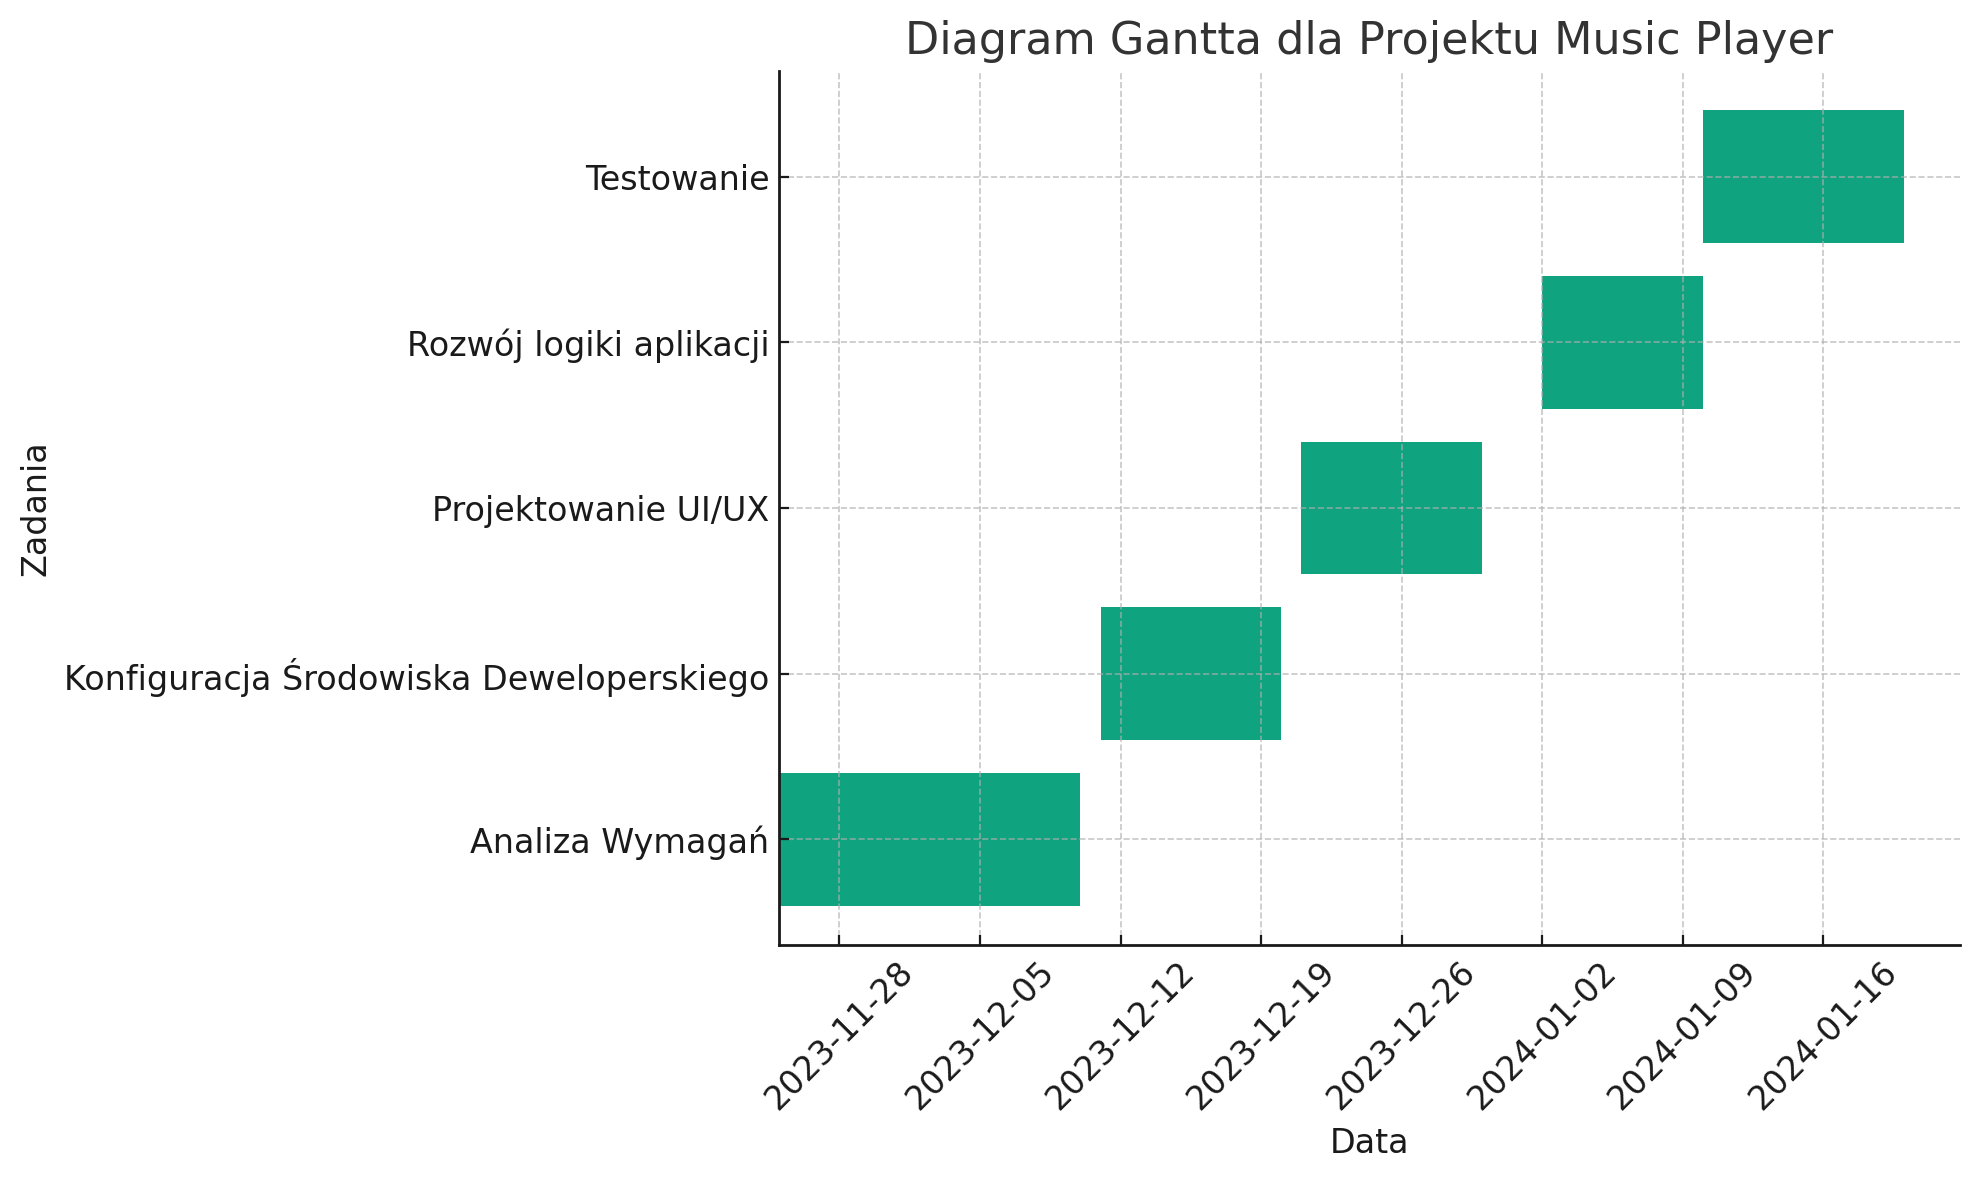
\includegraphics[height=200pt]{figures/diagram_gantta.png}
        \caption{{\footnotesize Schema bazy danych}}
	\end{center}
\end{figure}

{Szczegółowy opis zadań dla projektu:}

\begin{enumerate}
    \item \textbf{ Analiza Wymagań} (25.11.2023 - 10.12.2023)
    
        Czas na zrozumienie i zebranie kluczowych funkcjonalności wymaganych przez aplikację. Proces ten obejmuje przygotowanie listy narzędzi potrzebnych do wykonania projektu, analizę konkurencyjnych aplikacji. Jest to fundament, na którym opiera się cały projekt.
    \item \textbf{ Konfiguracja Środowiska Deweloperskiego} (11.12.2023 - 20.12.2023) 
    
    Ustanowienie odpowiedniego środowiska deweloperskiego jest kluczowe dla produktywności. W tym okresie zostało skonfigurowane IDE, zależności, docker, docker-compose, biblioteki oraz repozytorium Git, aby zapewnić płynny start i ciągłość prac nad projektem.
    \item \textbf{ Projektowanie UI/UX:} (21.12.2023 - 30.12.2023)
    
        Projekt interfejsu użytkownika (UI) oraz doświadczenia użytkownika (UX) ma bezpośredni wpływ na odbiór aplikacji przez użytkowników. W tym czasie budowany był cały główny interfejs UI by już na gotowej bazie okodować cała logikę aplikacji.
        \newpage

    \item \textbf{ Rozwój logiki aplikacji:} (02.1.2024 - 09.1.2024)

        Kluczowy etap rozwoju projektu, gdzie fokus położony był na implementację zaprojektowanego interfejsu użytkownika z właściwymi mechanizmami działania aplikacji. Ten okres pracy obejmował kodowanie głównych funkcji aplikacji, takich jak odtwarzanie muzyki, zarządzanie playlistami.
    \item \textbf{ Testowanie }  (10.01.2024 - 20.01.2024)
    
    Testowanie jest niezbędnym etapem w cyklu życia oprogramowania. W tym okresie aplikacja była testowana manualnie i poprawiana na bieżąco. W testowaniu pomagał również wcześniej stworzony skrypt CI/CD, który przy każdym zatwierdzeniu zmian automatycznie sprawdzał, czy aplikacja kompiluje się poprawnie.
    
\end{enumerate}

\section{Repozytorium i System Kontroli Wersji}

{Projekt jest rozwijany z użyciem systemu kontroli wersji Git, co pozwala na efektywną współpracę i śledzenie historii zmian. Repozytorium projektu znajduje się na GitHub pod adresem: \newline
\textbf{https://github.com/byko-dev/music-player}. Projekt będzie zamieszczony pod danym linkiem do dnia 31.03.2025. Dzięki wykorzystaniu Git, możliwe było efektywne zarządzanie kodem źródłowym.}

\section{Problemy i Trudności}
{W trakcie realizacji projektu Music Player napotkano różnorodne wyzwania. Jednym z nich było zapewnienie wysokiej jakości interfejsu użytkownika, co wymagało dokładnego planowania i testowania. Największym wyzwaniem okazało się stworzenie systemu do importu i eksportu danych z aplikacji. Zaplanowane wcześniej relacje w tabelach nie ułatwiały zadania, ponieważ program eksportował niechciane i często błędne dane, a podczas importu trudno było zachować relacje między tabelami. Dosyć szybko okazało się konieczne odejście od importu/eksportu tabeli Files, ponieważ była to operacja wymagająca i zasobożerna. Rozwiązaniem problemu okazało się stworzenie obiektów z prefixem 'Raw', które nie implementują relacji tabelarycznych.
}
\newpage
% ********** Rozdział 4 **********
\chapter{Prezentacja warstwy użytkowej projektu}

Projekt "Music Player" został zaprojektowany z myślą o zapewnieniu intuicyjnego, łatwego w obsłudze i estetycznie przyjemnego interfejsu użytkownika. W tej części dokumentacji szczegółowo omówimy poszczególne komponenty interfejsu, w tym layout, nawigację, funkcje dostępne dla użytkownika oraz ogólną koncepcję i filozofię stojącą za projektowaniem UI/UX. 


\begin{figure}[!ht]
	\begin{center}
	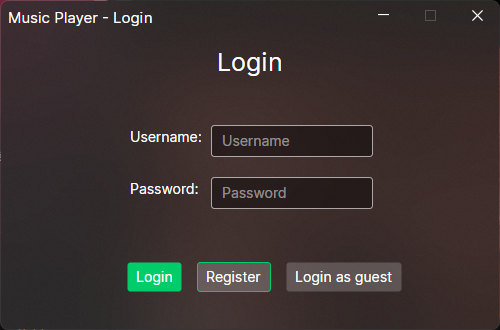
\includegraphics[height=200pt]{figures/login.png}
        \caption{{\footnotesize Formularz logowania}}
	\end{center}
\end{figure}

{Formularz logowania w aplikacji "Music Player" stanowi pierwszy punkt interakcji użytkownika z aplikacją, łącząc w sobie elegancję i prostotę. 
Tło formularza jest częściowo przezroczyste dzięki zastosowaniu efektu rozmycia, co sprawia, że prezentuje się ono za każdym razem inaczej, w zależności od tła znajdującego się pod naszą aplikacją. Pola "Username" i "Password" są intuicyjnie umieszczone w centralnym punkcie okna, co pozwala na szybkie i wygodne wprowadzenie danych przez użytkownika. Trzy przyciski akcji – "Login", "Register" oraz "Login as guest" – są wyraźnie oznaczone i zróżnicowane kolorystycznie, co nie tylko dodaje dynamiki wizualnej, ale także prowadzi użytkownika przez proces logowania krok po kroku.
}
\newpage

\begin{figure}[!ht]
	\begin{center}
	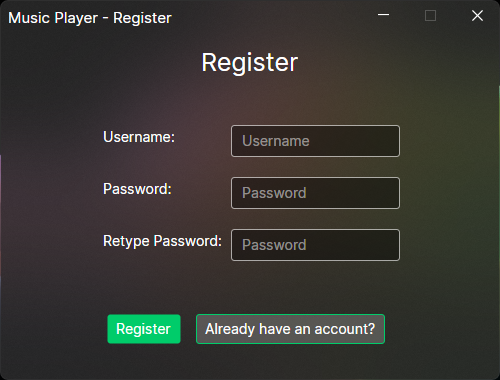
\includegraphics[height=240pt]{figures/register.png}
        \caption{{\footnotesize Formularz rejestracji}}
	\end{center}
\end{figure}

{Ekran rejestracji w aplikacji ma podobną konstrukcję do wcześniej wspomnianego ekranu logowania. Składa się z trzech głównych pól: 'Username', 'Password' oraz 'Retype Password', które są wyraźnie oznaczone i logicznie rozmieszczone, ułatwiając w ten sposób proces zakładania nowego konta. }

\begin{figure}[!ht]
	\begin{center}
	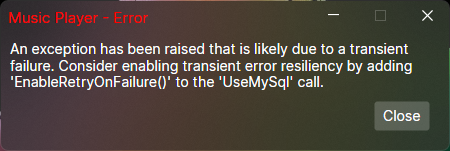
\includegraphics[]{figures/error_box.png}
        \caption{{\footnotesize Okno błędów}}
	\end{center}
\end{figure}

{
Okno błędu w aplikacji "Music Player" zostało zaprojektowane w celu przekazania ważnych informacji w sposób jasny i zwięzły. Treść okna błędu informuje o wyjątku, który został zgłoszony z powodu chwilowego problemu i sugeruje rozwiązanie techniczne, które może pomóc w jego rozwiązaniu.
Przycisk "Close" znajdujący się na dole okna jest wyraźnie zaznaczony i pozwala użytkownikowi szybko zamknąć komunikat błędu. Całość prezentuje się profesjonalnie i ma na celu ułatwienie szybkiego zidentyfikowania i rozwiązania problemu.
}

\newpage

\begin{figure}[h!]
  \centering
  \begin{minipage}{.53\textwidth}
    \centering
    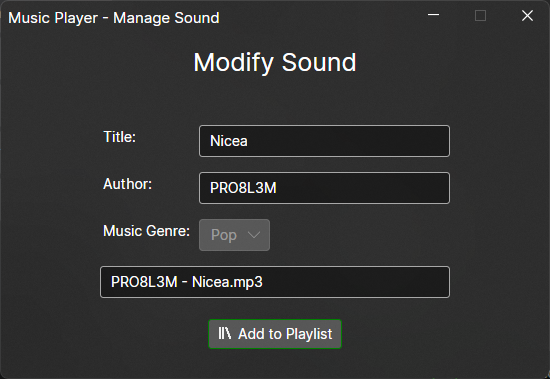
\includegraphics[width=.9\linewidth]{figures/modify1.png}
    \caption{{\footnotesize Okno edycji utworu - okno użytkownika}}
  \end{minipage}%
  \begin{minipage}{.55\textwidth}
    \centering
    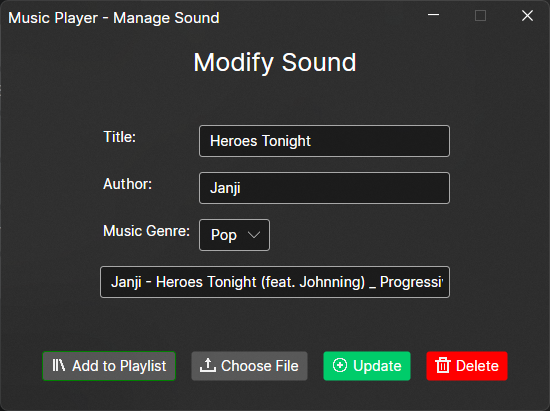
\includegraphics[width=.9\linewidth]{figures/modify2.png}
    \caption{{\footnotesize Okno edycji utowru - okno właściciela}}
  \end{minipage}
\end{figure}

{
Okna "Modify Sound" w aplikacji "Music Player" przedstawiają interfejs użytkownika umożliwiający zarządzanie informacjami o piosenkach. Są one dostosowane do różnych poziomów dostępu użytkownika, w zależności od tego, czy użytkownik dodał daną piosenkę do aplikacji.

Pierwsze okno jest przeznaczone dla użytkownika, który nie ma możliwości edycji informacji o piosence, ponieważ nie jest jej właścicielem. Prezentuje podstawowe informacje takie jak tytuł utworu ("Nicea"), autora ("PRO8L3M") oraz gatunek muzyczny ("Pop"). Na dole okna znajduje się przycisk "Add to Playlist", który pozwala na dodanie utworu do osobistej playlisty. Całość prezentuje się czysto i profesjonalnie, z zachowaniem spójnej kolorystyki i stylu.

Drugie okno jest dostępne dla użytkownika, który jest właścicielem piosenki i dlatego ma możliwość jej edycji. Użytkownik może zmieniać tytuł ("Heroes Tonight"), autora ("Janji") oraz gatunek muzyczny z dostępnego menu rozwijanego. W tym oknie dodane są dodatkowe opcje: przycisk "Choose File" umożliwia zmianę pliku muzycznego, "Update" służy do zapisania zmian, a "Delete" pozwala na usunięcie utworu z bazy danych aplikacji. Dodatkowo, utwór można dodać do playlisty za pomocą przycisku "Add to Playlist". Przyciski akcji są intuicyjnie zaprojektowane z użyciem symboli i kolorów, gdzie zielony symbolizuje akcję aktualizacji, a czerwony - usunięcie.

Oba okna są zaprojektowane z myślą o przejrzystości i łatwości użytkowania, przy jednoczesnym zachowaniu funkcjonalności i estetycznego wyglądu zgodnego z ogólnym motywem aplikacji.
}
\newpage

\begin{figure}[h!]
  \centering
  \begin{minipage}{.53\textwidth}
    \centering
    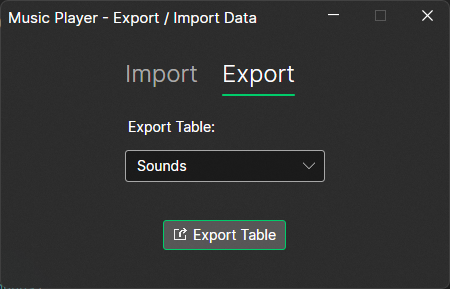
\includegraphics[width=.9\linewidth]{figures/export.png}
    \caption{{\footnotesize Okno eksportu danych}}
  \end{minipage}%
  \begin{minipage}{.55\textwidth}
    \centering
    
\includegraphics[width=.9\linewidth]{figures/import.png}
    \caption{{\footnotesize Okno importu danych}}
  \end{minipage}
\end{figure}

{
Okna importu i eksportu danych aplikacji "Music Player" są przejrzyste i funkcjonalne, umożliwiając użytkownikom łatwą migrację ich danych w formacie CSV, co jest standardem dla list utworów, playlist i informacji o użytkownikach.


\textbf{Okno eksportu danych:}
W oknie eksportu użytkownik ma możliwość wyeksportowania wybranej tabeli danych do pliku CSV. Proces jest prosty i intuicyjny – wystarczy wybrać interesującą tabelę z rozwijanego menu (np. "Sounds"), a następnie kliknąć przycisk "Export Table". To wyzwoli automatyczne pobieranie pliku CSV zawierającego wszystkie dane z wybranej tabeli. Ta funkcja jest szczególnie przydatna przy tworzeniu kopii zapasowych lub przenoszeniu danych między różnymi instancjami aplikacji.

\textbf{Okno eksportu danych:}
Okno importu danych oferuje użytkownikom możliwość załadowania danych z pliku CSV do aplikacji. Użytkownik może wybrać typ danych do importu (np. "Sounds", "Users", "Playlists") z rozwijanego menu. Pod menu znajduje się przewodnik po importowaniu, który krok po kroku informuje o sposobie importowania danych z różnych tabel. Aby zaimportować dane, użytkownik musi najpierw wybrać odpowiedni plik CSV z dysku, używając przycisku "Choose File", a następnie inicjować import przez kliknięcie "Import Table". Jest to krytyczna funkcja dla użytkowników, którzy chcą przywrócić dane lub zintegrować nowe kolekcje do swojej biblioteki.
}

\newpage

\begin{figure}[!ht]
	\begin{center}
	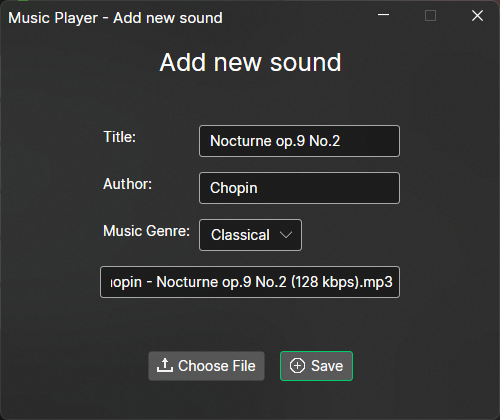
\includegraphics[]{figures/add_new_sound.png}
        \caption{{\footnotesize Formularz dodawania utworów}}
	\end{center}
\end{figure}

{Okno "Add new sound" w aplikacji "Music Player" jest przeznaczone do łatwego dodawania nowych utworów do biblioteki użytkownika. Użytkownicy mogą wprowadzić metadane dla każdego nowego dźwięku, takie jak tytuł utworu, autora oraz gatunek muzyczny z rozwijanego menu, gdzie można wybrać np. Classical, Pop, Rock, Jazz. Te pola pozwolą na lepszą organizację i wyszukiwanie w przyszłości.

Pole na dole, gdzie wyświetlana jest nazwa pliku, pokazuje wybrany utwór do dodania, który użytkownik załadował przez przycisk "Choose File". Po wybraniu pliku, utwór może być dodany do biblioteki aplikacji za pomocą przycisku "Save", który jest wyraźnie widoczny i łatwy do zlokalizowania.
Proces dodawania jest intuicyjny i zaprojektowany tak, aby maksymalnie uproszczać zarządzanie kolekcją muzyki użytkownika.}

\newpage

\begin{figure}[!ht]
	\begin{center}
	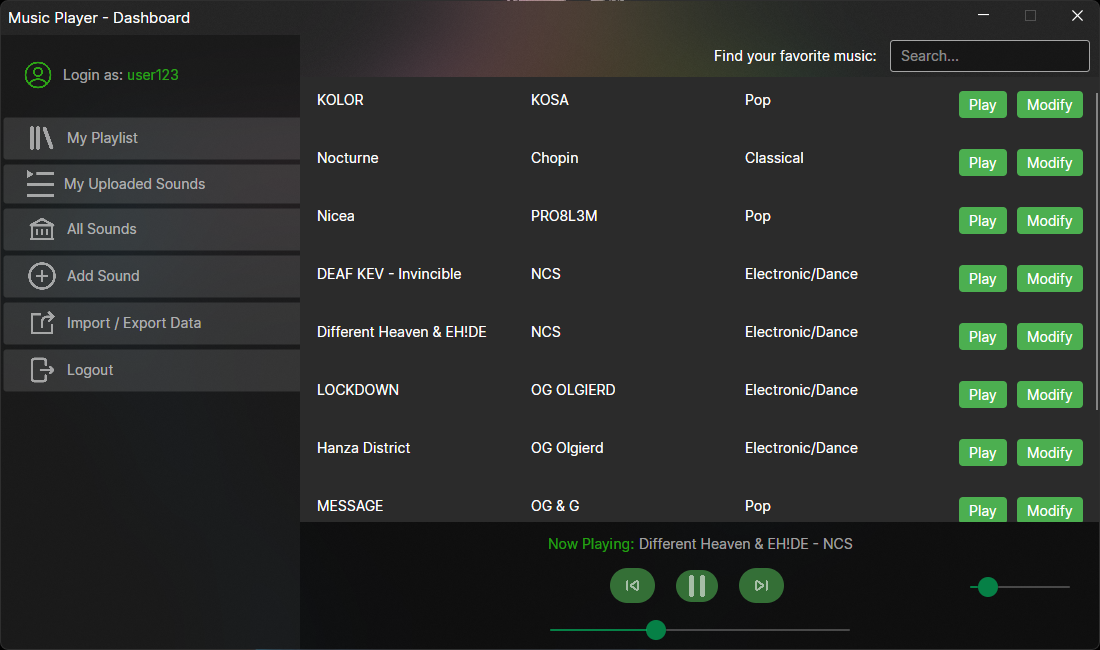
\includegraphics[width=500pt]{figures/main1.png}
        \caption{{\footnotesize Główne okno aplikacji}}
	\end{center}
\end{figure}

{
Główne okno aplikacji "Music Player" to centrum dowodzenia dla użytkownika, gdzie może zarządzać swoją muzyczną biblioteką i odtwarzaniem. Na lewym pasku bocznym znajduje się intuicyjne menu nawigacyjne z ikonami, które umożliwiają szybki dostęp do różnych sekcji aplikacji, takich jak "My Playlist", "My Uploaded Sounds", "All Sounds", a także opcje do dodawania nowych dźwięków i importu/eksportu danych. Na dole znajduje się opcja "Logout", która pozwala użytkownikowi bezpiecznie wylogować się z aplikacji.

W centralnej części okna znajduje się lista utworów z ich tytułami, autorami i gatunkami muzycznymi. Każdy wpis na liście ma przypisane przyciski "Play" i "Modify", które pozwalają odpowiednio na odtwarzanie wybranego utworu oraz jego edycję – ta druga opcja jest dostępna tylko dla utworów dodanych przez zalogowanego użytkownika.

Na górze tego panelu znajduje się pasek wyszukiwania, który umożliwia szybkie znalezienie ulubionej muzyki według nazwy utworu, wykonawcy lub gatunku.

Dolna część ekranu to dedykowany pasek odtwarzacza z podstawowymi przyciskami sterowania odtwarzaniem (play, pause, skip), a także pasek postępu, który wizualnie pokazuje postęp aktualnie odtwarzanego utworu. Ponadto wyświetlana jest nazwa aktualnie odtwarzanego utworu, co pozwala użytkownikowi na szybką identyfikację odtwarzanej kompozycji.

Całość interfejsu utrzymana jest w ciemnej kolorystyce, co jest przyjemne dla oka i nie męczy wzroku podczas dłuższego korzystania z aplikacji w różnych warunkach oświetleniowych.

}

\newpage

\begin{figure}[!ht]
	\begin{center}
	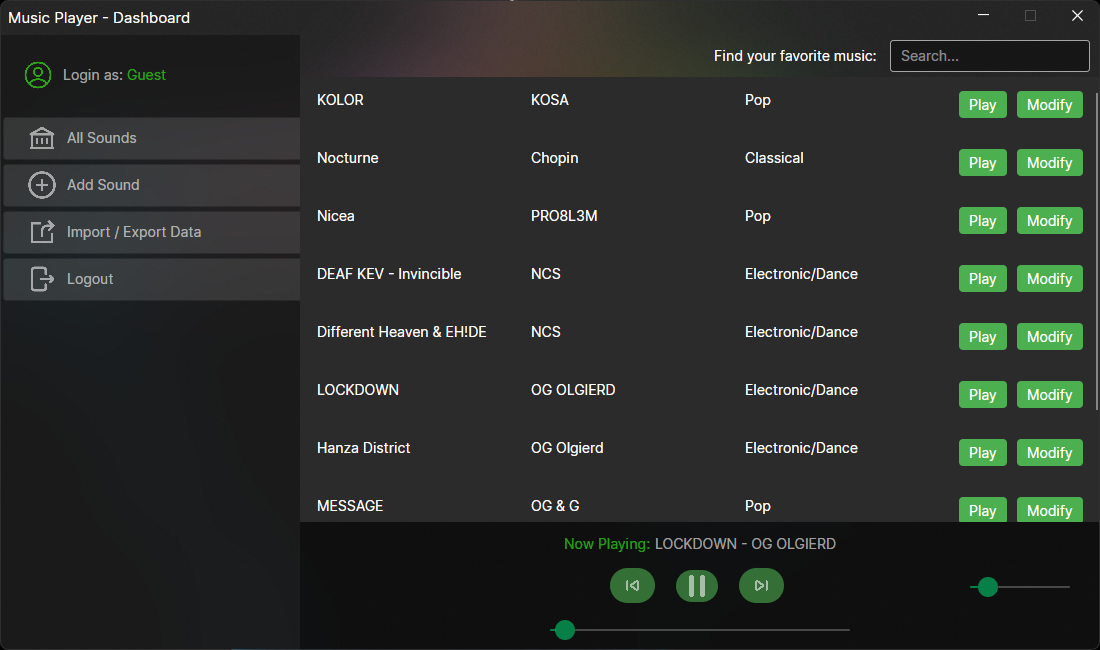
\includegraphics[width=500pt]{figures/main_guest.png}
        \caption{{\footnotesize Główne okno aplikacji - widok gościa}}
	\end{center}
\end{figure}

{W porównaniu do wcześniejszego okna dashboardu dla zalogowanego użytkownika, obecne okno dla gościa prezentuje się bardzo podobnie, z tą różnicą, że nie zawiera opcji "My Playlist" ani "My Uploaded Sounds". To wskazuje na ograniczoną funkcjonalność dostępną dla użytkowników, którzy nie są zalogowani lub korzystają z aplikacji jako goście.

Status logowania na górze okna zmienia się z konkretnego identyfikatora użytkownika (np. user123) na ogólne oznaczenie "Guest", co podkreśla, że użytkownik nie jest obecnie zalogowany i korzysta z aplikacji w ograniczonym zakresie. Użytkownik gość ma dostęp do ogólnej listy utworów w sekcji "All Sounds", może przeszukiwać dostępną muzykę i korzystać z funkcji odtwarzania, ale nie posiada możliwości modyfikacji listy utworów ani zarządzania własnymi dźwiękami. Może również wyeksportować/importować dane i wylogować się z systemu, co wskazuje na pewne podstawowe interakcje, które są dostępne dla każdego, kto korzysta z aplikacji.}

% ********** Koniec rozdziału **********

\newpage
% ********** Rozdział 4 **********
\chapter{Podsumowanie}

Projekt Music Player, który rozpoczął się od ambitnych założeń, nie tylko spełnił pierwotne oczekiwania, ale także znacznie je przekroczył. W miarę rozwoju projektu, udało się zaimplementować szereg dodatkowych elementów, które podniosły wartość aplikacji. Dzięki wprowadzeniu konfiguracji GitHub Actions, proces wdrażania i ciągłej integracji stał się bardziej efektywny i automatyczny, a zastosowanie docker-compose pozwoliło na sprawną konfigurację środowiska deweloperskiego.

Podczas fazy developmentu, opracowano i zintegrowano solidną bazę danych SQL, co było znaczącym krokiem naprzód w zakresie zarządzania i dostępności danych. Ta zmiana zapewniła lepszą skalowalność aplikacji i otworzyła drzwi do dalszego rozszerzenia funkcjonalności.

Patrząc w przyszłość, plany rozwojowe aplikacji Music Player obejmują wprowadzenie opcji tworzenia spersonalizowanych playlist przez użytkowników, co uczyni aplikację jeszcze bardziej interaktywną i personalną. Ponadto, rozważa się możliwość wyboru między różnymi bazami danych z muzyką, dając użytkownikom jeszcze szerszy dostęp do różnorodnych utworów i gatunków muzycznych. Prace nad rozbudową opcji konfiguracji interfejsu użytkownika oraz funkcji aplikacji są także wizją, która może przekształcić Music Player w jeszcze bardziej zaawansowane narzędzie, dostosowane do potrzeb i preferencji szerokiej grupy odbiorców. Znaczący nacisk położono na estetykę UI, co przełożyło się na przyjemność użytkowania i pozytywne doświadczenia w interakcji z aplikacją. Staranne projektowanie UI, zgodne z najnowszymi trendami w designie, sprawia, że aplikacja wyróżnia się na tle innych odtwarzaczy muzycznych, oferując intuicyjność oraz wizualny komfort. Nowoczesny interfejs użytkownika, opracowany z myślą o zapewnieniu najlepszych wrażeń, jest jednym z kluczowych osiągnięć projektu i stanowi solidną platformę dla planowanych rozszerzeń funkcjonalności Music Player'a.

Podsumowując, realizacja projektu Music Player przeszła długą drogę od początkowych założeń po wdrożenie praktycznych i zaawansowanych rozwiązań. Z sukcesem zbudowano podstawy, które nie tylko zapewniają stabilną i funkcjonalną aplikację, ale także stwarzają mocne fundamenty pod przyszłą ekspansję i innowacje.



% ********** Koniec rozdziału **********


\newpage

% *************** Bibliografia ***************
\begin{thebibliography}{6}
\addcontentsline{toc}{chapter}{Bibliografia}
%dodanie wpisu do spisu bibliograficznego

  

\bibitem{etykieta1}Jacek Matulewski, {\it C\#: lekcje programowania: praktyczna nauka programowania dla platform .NET i .NET Core}, Helion, Gliwice 2021.
\bibitem{etykieta2}Joseph  Albahari, Eric Johannsen, {\it C\# 8.0 w pigułce}, Helion, Gliwice, 2021.
\bibitem{etykieta3}R. S. Miles, {\it C\#: zacznij programować!}, Helion, Gliwice, 2020.
\bibitem{etykieta4}Włodzimierz Gajda, {\it Git : rozproszony system kontroli wersji}, Helion, Gliwice, 2013.
\bibitem{etykieta4}A. Stellman, J. Greene, {\it C\#. Rusz głową!}, Helion, Gliwice, 2022.
\end{thebibliography}
\newpage
 
% *************** Zakończenie ***************
% *************** Zakończenie ***************

%***************************************************************************************
% W tym miejscu znajdują się polecenia odpowiedzialne za tworzenie
% spisu ilustracji, spisu treści oraz streszczenia pracy
%***************************************************************************************

%spis rysunków
\addcontentsline{toc}{chapter}{Spis rysunków}
\listoffigures
\newpage

%spis tablic
\addcontentsline{toc}{chapter}{Spis tablic}
\listoftables
\newpage

% %streszczenie
% \addcontentsline{toc}{chapter}{Streszczenie}
% \noindent
% {\footnotesize{}\textbf{Wyższa Szkoła Informatyki i Zarządzania z siedzibą w Rzeszowie\\
% Kolegium Informatyki Stosowanej}
% \vspace{30pt}

% \begin{center}
% \textbf{Streszczenie pracy dyplomowej inżynierskiej}\\
% \temat
% \end{center}

% \vspace{30pt}
% \noindent
% \textbf{Autor: \autor
% \\Promotor: \promotor
% \\Słowa kluczowe: tutaj umieść słowa kluczowe}
% \vspace{40pt}
% \\Treść streszczenia, czyli kilka zdań dotyczących treści pracy dyplomowej w języku polskim.
% \vspace{80pt}

% \noindent
% \textbf{The University of Information Technology and Management in Rzeszow\\
% Faculty of Applied Information Technology}
% \vspace{30pt}

% \begin{center}
% \textbf{Thesis Summary\\}
% Tytuł pracy w języku angielskim
% \end{center}

% \vspace{30pt}
% \noindent
% \textbf{Author: \autor
% \\Supervisor: \promotor
% \\Key words: tutaj umieść słowa kluczowe}
% \vspace{40pt}
% \\Treść streszczenia, czyli kilka zdań dotyczących treści pracy dyplomowej w języku angielskim - tłumaczenie tekstu z języka polskiego.
% }

% *************** Koniec pliku back.tex ***************


\end{document}
% *************** Koniec pliku szablon.tex ***************
